\begin{circuitikz}[scale=1]
\def\xspacing{2}
\def\xstart{0}
\def\yspacing{2}	
\def\ystart{0}

%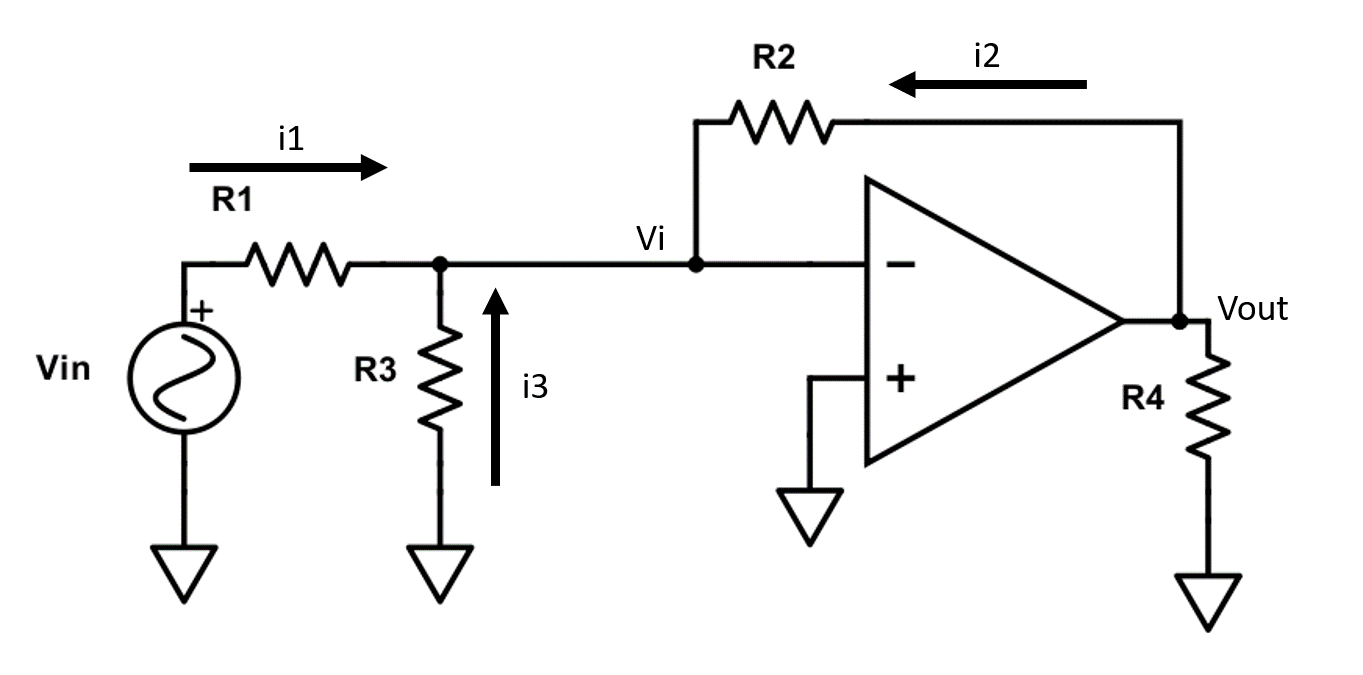
\includegraphics[width=0.5\textwidth]{imagenes/xxx.png}




%dibujo malla izquierda
\draw   						(\xstart, \ystart) node[ground]{}
		to [vsourcesin]	 	(\xstart, \ystart + \yspacing)
		to [R=$R_1$, i>^=$i_1$] (\xstart + \xspacing, \ystart + \yspacing)
		to [R=$R_3$, i<^=$i_3$] (\xstart + \xspacing, \ystart)
		to (\xstart + \xspacing, \ystart) node[ground]{}

%dibujo opamp
%el opamp tiene la misma altura que scale, y las patitas - y + estan en .25*scale y .75*scale
%nos queda - en ystart+yspacing y + en ystart+spacing-0.5

		(\xstart + 3*\xspacing, \ystart + \yspacing - .5) node[op amp] (opamp) {}

%dibujo conexiones a opamp
	 						   (\xstart + \xspacing, \ystart + \yspacing)
		to [short]			  (opamp.-)
								(opamp.+)
		to [short]			  ($(opamp.+)+(0,-\yspacing + 1)$) node[ground]{}	%se me va la patita
								(\xstart + 2*\xspacing, \ystart + 1*\yspacing)
		to [short, *-]		  (\xstart + 2*\xspacing, \ystart + 1.7*\yspacing)
		to [R=$R_2$, i<^=$i_2$] (\xstart + 4*\xspacing, \ystart + 1.7*\yspacing)
		to [short, -*]		  (\xstart + 4*\xspacing, \ystart + 1*\yspacing -.5)
		to [short]			  (opamp.out)
								(\xstart + 4*\xspacing, \ystart + 1*\yspacing -.5)
		to [R=$R_4$]			(\xstart + 4*\xspacing, \ystart) node[ground]{};


\end{circuitikz}
